\documentclass[12pt,a4paper]{scrartcl}

\usepackage[a4paper, left=2cm, right=1cm, bottom=1cm, top=1cm, includeheadfoot]{geometry}
\usepackage[ngerman]{babel}
\usepackage[utf8]{inputenc} % comment this if you uncomment utf8x
%\usepackage[utf8x]{inputenc} % uncomment this if there are problems with 'ä', 'ü', 'ö'
\usepackage{ucs}
\usepackage[usenames,dvipsnames]{xcolor}
\usepackage[fleqn]{amsmath}
\usepackage{amsfonts}
\usepackage{amssymb}
\usepackage{color}
\usepackage{listings}
\usepackage{hyperref}
\usepackage{amsfonts}
\usepackage{listings}
\usepackage{scrpage2}
\usepackage{graphicx}


\definecolor{mygray}{rgb}{0.9,0.9,0.9}
\lstset{language=[Visual]Basic, morekeywords={param, local}}


\lstset{
   literate={ö}{{\"o}}1
           {ä}{{\"a}}1
           {ü}{{\"u}}1
           {ß}{{\ss}}1
           {é}{{\'e}}1,
   inputencoding=ansinew,
   extendedchars=true,
   basicstyle=\scriptsize\ttfamily,
   numberstyle=\scriptsize,
   breaklines=true,
   tabsize=2,
   numbersep=5pt
}
\lstdefinestyle{customcpp}{
   language=C++,
   backgroundcolor=\color{mygray},
   numbers=left,
   keywordstyle=\color{blue}\bfseries,
   stringstyle=\color{BrickRed}\ttfamily,
   commentstyle=\color{OliveGreen}\ttfamily,
   showspaces=false,
   showstringspaces=false,
   showtabs=false
}
\lstdefinestyle{customoutput}{
   backgroundcolor=\color{mygray},
   numbers=none,
   showspaces=false,
   showtabs=false
}

\newcommand{\sourceCode}[1]{\lstinputlisting[style=customcpp]{#1}} %beinhaltet alle benötigten Packages etc.
\begin{document}
\graphicspath{{./}}

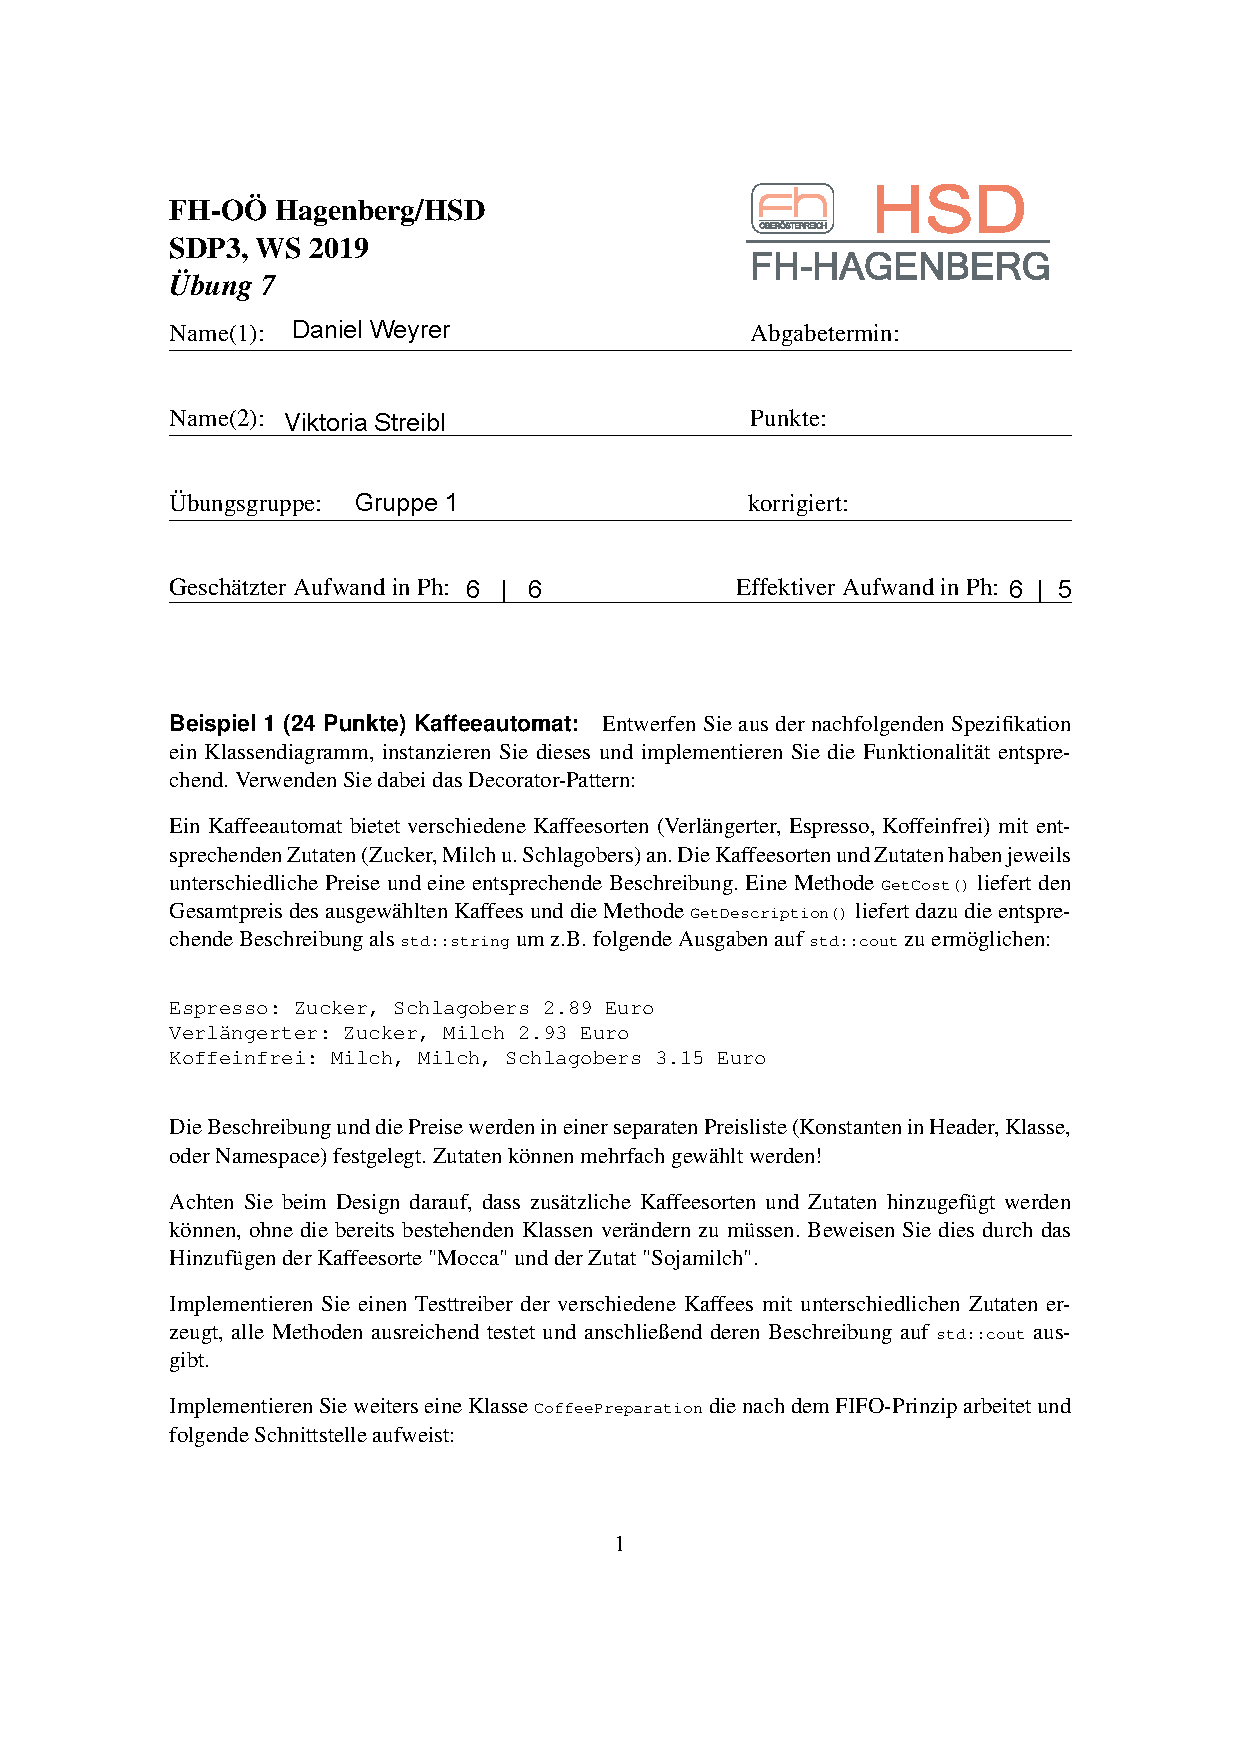
\includepdf[pages=-]{../Angabe.pdf}

\title{SDP - Exercise 07} % Übungsname und Nummer angeben
\subtitle{winter semester 2019/20} % Semester angeben oder auskommentieren, falls nicht erwünscht
\author{
Viktoria Streibl - S1810306013\\
  Daniel Weyrer - S1820306044
} % Autorenname
\date{\today} % Das heutige Datum automatisch einfügen

\maketitle % Titelseite erstellen

\newpage
\tableofcontents % Inhaltsverzeichnis erstellen
\newpage

\ihead{Viktoria Streibl}
\ohead{Daniel Weyrer}
\chead{SDP3-UE Uebung 07}

\section{Organizational}
\subsection{Team}
\begin{itemize}
	\item Viktoria 	Streibl 		- 	S1810306013
	\item Daniel 	Weyrer		-	S1820306044
\end{itemize}

\subsection{Roles and responsibilities}
\subsubsection{Jointly}
\begin{itemize}
	\item Planning
	\item Documentation
	\item Systemdocumentation
\end{itemize}

\subsubsection{Viktoria Streibl}
\begin{itemize}
	\item Object
	\item Pricelist
	\item Coffee Sorts
	\item Ingredient Sorts		
\end{itemize}

\subsubsection{Daniel Weyrer}
\begin{itemize}
	\item Coffeemachine
	\item TestDriver
	\item CoffeePreparation
	\item Ingredient
\end{itemize}

\subsection{Effort}

\subsubsection {Viktoria Streibl}
\begin{itemize}
	\item estimated: 6 ph 
	\item actually: 5 ph
\end{itemize}

\subsubsection {Daniel Weyrer}
\begin{itemize}
	\item estimated: 6 ph 
	\item actually: 6 ph
\end{itemize}

\section{Requirenment Definition(System Specification)}
This Coffeemachine should work like a normal Coffeemachine. It is a simulation to order different sort of coffee and add several ingredients. Depending on the selection the price will be displayed.

\section{System Design}
\subsection{Classdiagram}
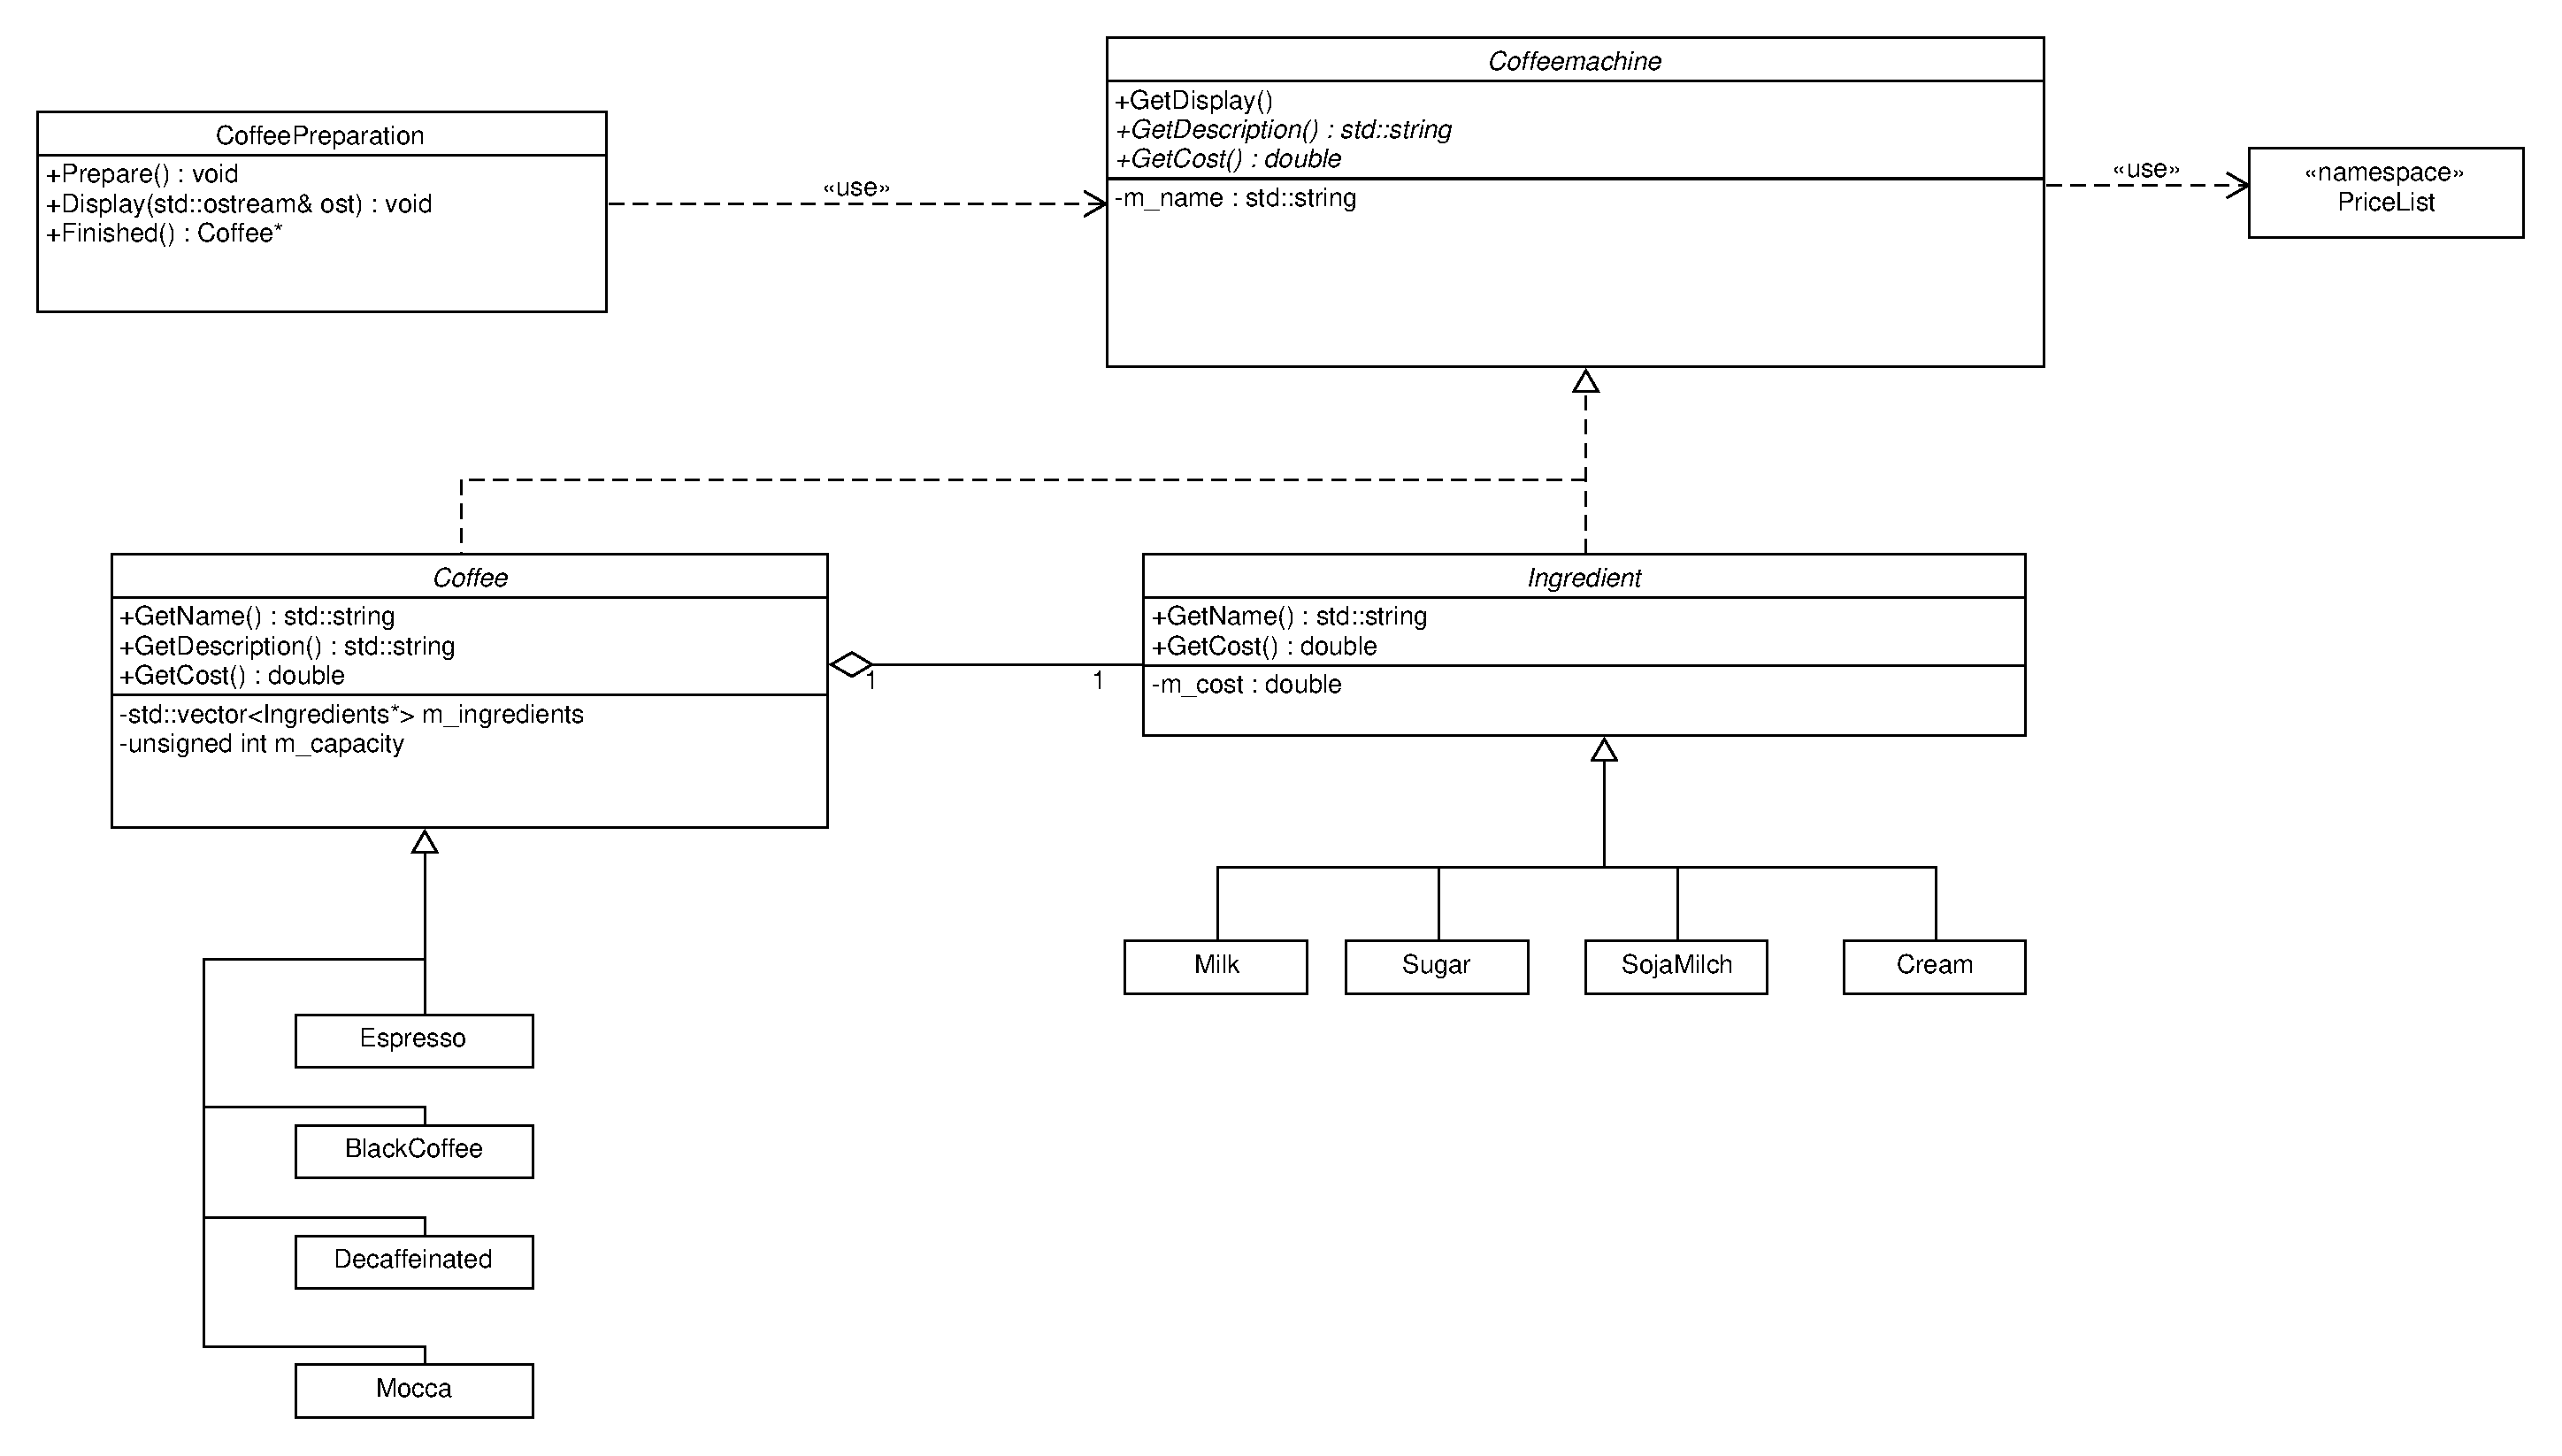
\includegraphics[scale=0.40, angle=90]{../ClassDiagram.pdf}

\subsection{Design Decisions}
\subsubsection{PriceList}
We decided to use an extra file to manage the different prices. This makes it easier to add change the prices afterwards.

\section{Component Design}
\subsection{CoffeePreparation}
It contains following Methods:
\begin{itemize}
	\item Prepare
	\item Display
	\item Finished
\end{itemize}


\subsection{Coffeemachine}
It contains following Methods:
\begin{itemize}
	\item GetDescription
	\item GetCost
	\item GetName
\end{itemize}

\subsection{Pricelist}
It contains a namespace where the prices of the different ingredients are declared.

\subsection{Ingredient}

\subsection{Coffee Sorts}
There are different kinds of coffee, the following are implemented:
\begin{itemize}
	\item Espresso
	\item Black Coffee
	\item Decaffeinated
	\item Mocca
\end{itemize}

\subsection{Ingredient Sorts}
There are different kinds of coffee, the following are implemented:
\begin{itemize}
	\item Milk
	\item Sugar
	\item Cream
	\item Soja Milk
\end{itemize}

They also have following methods:
\begin{itemize}
	\item GetDescription
	\item GetCost
\end{itemize}

\newpage

\section{Source Code}

\subsection{CoffeePreparation}
\subsubsection{CoffeePreparation.h}
\sourceCode{../../CoffeeMachine/CoffeeMachine/CoffeePreparation.h}
\subsubsection{CoffeePreparation.cpp}
\sourceCode{../../CoffeeMachine/CoffeeMachine/CoffeePreparation.cpp}
\newpage

\subsection{Coffeemachine}
\subsubsection{Coffeemachine.h}
\sourceCode{../../CoffeeMachine/CoffeeMachine/Coffeemachine.h}
\subsubsection{Coffeemachine.cpp}
\sourceCode{../../CoffeeMachine/CoffeeMachine/CoffeeMachine.cpp}
\newpage

\subsection{Espresso}
\subsubsection{Espresso.h}
\sourceCode{../../CoffeeMachine/CoffeeMachine/Espresso.h}
\subsubsection{Espresso.cpp}
\sourceCode{../../CoffeeMachine/CoffeeMachine/Espresso.cpp}
\newpage

\subsection{BlackCoffee}
\subsubsection{BlackCoffee.h}
\sourceCode{../../CoffeeMachine/CoffeeMachine/BlackCoffee.h}
\subsubsection{BlackCoffee.cpp}
\sourceCode{../../CoffeeMachine/CoffeeMachine/BlackCoffee.cpp}
\newpage

\subsection{Decaffeinated}
\subsubsection{Decaffeinated.h}
\sourceCode{../../CoffeeMachine/CoffeeMachine/Decaffeinated.h}
\subsubsection{Decaffeinated.cpp}
\sourceCode{../../CoffeeMachine/CoffeeMachine/Decaffeinated.cpp}
\newpage

\subsection{Mocca}
\subsubsection{Mocca.h}
\sourceCode{../../CoffeeMachine/CoffeeMachine/Mocca.h}
\subsubsection{Mocca.cpp}
\sourceCode{../../CoffeeMachine/CoffeeMachine/Mocca.cpp}
\newpage

\subsection{Ingredient}
\subsubsection{Ingredient.h}
\sourceCode{../../CoffeeMachine/CoffeeMachine/Ingredient.h}
\subsubsection{Ingredient.cpp}
\sourceCode{../../CoffeeMachine/CoffeeMachine/Ingredient.cpp}
\newpage

\subsection{Milk}
\subsubsection{Milk.h}
\sourceCode{../../CoffeeMachine/CoffeeMachine/Milk.h}
\subsubsection{Milk.cpp}
\sourceCode{../../CoffeeMachine/CoffeeMachine/Milk.cpp}
\newpage

\subsection{Sugar}
\subsubsection{Sugar.h}
\sourceCode{../../CoffeeMachine/CoffeeMachine/Sugar.h}
\subsubsection{Sugar.cpp}
\sourceCode{../../CoffeeMachine/CoffeeMachine/Sugar.cpp}
\newpage

\subsection{Cream}
\subsubsection{Cream.h}
\sourceCode{../../CoffeeMachine/CoffeeMachine/Cream.h}
\subsubsection{Cream.cpp}
\sourceCode{../../CoffeeMachine/CoffeeMachine/Cream.cpp}
\newpage

\subsection{SojaMilk}
\subsubsection{SojaMilk.h}
\sourceCode{../../CoffeeMachine/CoffeeMachine/SojaMilk.h}
\subsubsection{SojaMilk.cpp}
\sourceCode{../../CoffeeMachine/CoffeeMachine/SojaMilk.cpp}
\newpage

\subsection{PriceList}
\subsubsection{Pricelist.h}
\sourceCode{../../CoffeeMachine/CoffeeMachine/Pricelist.h}
\newpage

\subsection{TestDriver}
\sourceCode{../../CoffeeMachine/CoffeeMachine/TestDriver.cpp}
\newpage

\end{document}